\documentclass[10pt]{article}

\usepackage[utf8]{inputenc}
\usepackage{latexsym,amsfonts,amssymb,amsthm,amsmath}
\setlength{\parindent}{0in}
\setlength{\parskip}{\baselineskip}
\setlength{\oddsidemargin}{0in}
\setlength{\textwidth}{6.5in}
\setlength{\textheight}{8.8in}
\setlength{\topmargin}{0in}
\setlength{\headheight}{18pt}

\usepackage[a4paper,margin=1in,footskip=0.25in]{geometry}

\usepackage{listings}
\usepackage{color} %red, green, blue, yellow, cyan, magenta, black, white
\definecolor{mygreen}{RGB}{28,172,0} % color values Red, Green, Blue
\definecolor{mylilas}{RGB}{170,55,241}

\usepackage{graphicx}
\graphicspath{{../writeup/}}

\def\code#1{\texttt{#1}}

\usepackage[colorlinks=true, urlcolor=blue, linkcolor=red]{hyperref}

\title{PHYS 410 Homework 1}
\author{Gavin Pringle, 56401938}

%%%%%%%%%%%%%%%%%%%%%%%%%%%%%%%%%%%%%%%%%%%%%%%%%%%%%%%%%%%%%%%%%%%%%%%%%%%%%%%%%%%%%%%%%%%%%%%%%%%%%%%
% Start of document
%%%%%%%%%%%%%%%%%%%%%%%%%%%%%%%%%%%%%%%%%%%%%%%%%%%%%%%%%%%%%%%%%%%%%%%%%%%%%%%%%%%%%%%%%%%%%%%%%%%%%%%
\begin{document}

\maketitle

\lstset{language=Matlab,%
    %basicstyle=\color{red},
    breaklines=true,%
    morekeywords={matlab2tikz},
    keywordstyle=\color{blue},%
    morekeywords=[2]{1}, keywordstyle=[2]{\color{black}},
    identifierstyle=\color{black},%
    stringstyle=\color{mylilas},
    commentstyle=\color{mygreen},%
    showstringspaces=false,%without this there will be a symbol in the places where there is a space
    numbers=left,%
    numberstyle={\tiny \color{black}},% size of the numbers
    numbersep=9pt, % this defines how far the numbers are from the text
    emph=[1]{for,end,break},emphstyle=[1]\color{red}, %some words to emphasise
    %emph=[2]{word1,word2}, emphstyle=[2]{style},    
}

%%%%%%%%%%%%%%%%%%%%%%%%%%%%%%%%%%%%%%%%%%%%%%%%%%%%%%%%%%%%%%%%%%%%%%%%%%%%%%%%%%%%%%%%%%%%%%%%%%%%%%%
% Introduction
%%%%%%%%%%%%%%%%%%%%%%%%%%%%%%%%%%%%%%%%%%%%%%%%%%%%%%%%%%%%%%%%%%%%%%%%%%%%%%%%%%%%%%%%%%%%%%%%%%%%%%%
\subsection*{Introduction}

In this homework assignment, two methods for solving nonlinear equations numerically via root finding 
are explored: bisection and Newton's method. In order to do this, two problems are provided. The first 
problem involves the 1-dimesional case where the roots of a nonlinear function are found using a hybrid 
algorithm that first employs bisection followed by Newton's method. The second problem involves the 
d-dimensional case where a nonlinear system is solved using a d-dimensional Newton iteration. 

In both problems it is assumed that the function and its derivative in problem 1 as well as the system of 
equations and its Jacobian in problem 2 are hard-coded as Matlab functions. Specifically, a polynomial
of order 10 is provided for the first question and a nonlinear system of three variables is provided 
for the second question. 

\pagebreak

%%%%%%%%%%%%%%%%%%%%%%%%%%%%%%%%%%%%%%%%%%%%%%%%%%%%%%%%%%%%%%%%%%%%%%%%%%%%%%%%%%%%%%%%%%%%%%%%%%%%%%%
% Problem 1 - Hybrid Algorithm
%%%%%%%%%%%%%%%%%%%%%%%%%%%%%%%%%%%%%%%%%%%%%%%%%%%%%%%%%%%%%%%%%%%%%%%%%%%%%%%%%%%%%%%%%%%%%%%%%%%%%%%
\subsection*{Problem 1 - Hybrid Algorithm}

\subsubsection*{Review of Theory}

\textbf{Bisection}, also referred to as binary search, is a method used for solving nonlinear equations of the 
form $f(x)=0$ for the 1-dimensional case or $\mathbf{f}(\mathbf{x})=\mathbf{0}$ for the d-dimensional case. The
bisection algorithm involves bisecting a search interval and checking whether the root is above or 
below the bisector. The search interval is then bisected again in the new interval where the root lies, 
and again it is determined whether the root is above or below the new bisector. This process then repeats
until the root is determined to be in an interval of small enough tolerance. 

For the 1-dimensional bisection algorithm, it is assumed that there is a root of $f(x)=0$ in the interval
$x_{min} \leq x \leq x_{max}$. From this, it follows that $f(x_{min})f(x_{max}) \leq 0$. As previously 
described, the interval $[x_{min}, x_{max}]$ which has width $\delta x_0 = x_{max} - x_{min}$ is
successively divided into smaller intervals of width $\delta x_1 = \delta x_0/2$, 
$\delta x_2 = \delta x_0/4$, $\delta x_3 = \delta x_0/8$, \ldots each of which contains the root which is 
checked using the condition $f({x_{min}}^{(n)})f({x_{max}}^{(n)}) \leq 0$. This process is continued until 
interval is suitably small, which is verified by checking the relative error given by the formula
$\frac{| \delta x^{(n)} |}{| x^{(n+1)} |} \leq \epsilon$.

\textbf{Newton's method} is another method used for solving nonlinear equations of the form $f(x)=0$ for the 
1-dimensional case or $\vec{f}(\vec{x})=\vec{0}$ for the d-dimensional case. Newton's method does not 
require an interval wherein the root lies but rather a "good" initial guess as to where the root is near.
Whether or not the guess is "good" depends on the specific problem at hand.

In Newton's method, we let $x^*$ be a root of $f(x)$. From the Taylor expansion,
$$0 \approx f(x^{(n)}) + (x^* - x^{(n)})f'(x^{(n)})$$
Letting $x^{(n+1)} = x^*$, we can rearrange to get
$$x^{(n+1)} = x^{(n)} - \frac{f(x^{(n)})}{f'(x^{(n)})}$$
For the 1-dimensional Newton's method algorithm, the above equation can be successively applied to yield a 
closer and closer approximation to the true $x^*$. The process can again be stopped when a suitable precision
is achieved, calculated using the formula 
$$\frac{| \delta x^{(n)} |}{| x^{(n+1)} |} = \frac{| x^{(n+1)}-x^{(n)} |}{| x^{(n+1)} |} \leq \epsilon$$

\subsubsection*{Numerical Approach}

Both of the 1-dimensional bisection algorithm and 1-dimensional Newton's method are used in this problem to 
create a hybrid algorithm that first employs bisection to an intermediate tolerance followed by Newton's method to
a final tolerance in order to find the root of an arbitrary function was in the interval $[x_{min}, x_{max}]$.
The algorithm was implemented as a function (as per the homework instructions):
\begin{verbatim}
function x = hybrid(f, dfdx, xmin, xmax, tol1, tol2)
\end{verbatim}
where \code{x} is the returned value of the calculated root, \code{f} is the function for which the location
of the root is sought, \code{dfdx} is the derivative of said function, \code{xmin} is the initial interval 
minimum, \code{xmax} is the initial interval maximum, \code{tol1} is the relative convergence criterion for
bisection, and \code{tol2} is the relative convergence criterion for Newton iteration.

In order to test the function \code{hybrid(f, dfdx, xmin, xmax, tol1, tol2)}, the polynomial 
$$f(x) = 512x^{10}-5120x^9 + 21760x^8-51200x^7 + 72800x^6-64064x^5 + 34320x^4-10560x^3 + 1650x^2-100x + 1$$
and its derivative were both implemented as Matlab functions to pass as parameters. The online graphing 
calculator Desmos was used to graph the function in order to see where the roots are in order to find search intervals
for each root of $f(x)$ in the interval $[0,2]$. For testing purposes \code{tol1} was set to $10^{-4}$ and 
\code{tol2} was set to $10^{-12}$ as per the homework instructions on relative precision. Refer to Appendix C 
for the full Matlab test script. 

\subsubsection*{Implementation}

The function \code{hybrid(f, dfdx, xmin, xmax, tol1, tol2)} first employs bisection via a while loop to a 
precision of \code{tol1}. The middle of the final bisection interval is passed as the starting point for the 
Newton's method algorithm which then computes the root to a precision of \code{tol2} via another while loop. 
A loop iteration counter is utilized for both the bisection and Newton's method loops that causes the function
to immediately return \code{NaN} if either loop exceed 50 iterations.

Refer to Appendix A for the full Matlab script.

\subsubsection*{Results}

Using the script \code{test.m} shown in Appendix C, the roots of $f(x)$ were computed using the hybrid algorithm
as 
\begin{verbatim}
roots(1) = 0.012311659405
roots(2) = 0.108993475812
roots(3) = 0.292893218813
roots(4) = 0.546009500260
roots(5) = 0.843565534960
roots(6) = 1.156434465042
roots(7) = 1.707106781183
roots(8) = 1.891006524190
roots(9) = 1.453990499747
roots(10) = 1.987688340584
\end{verbatim}

Plugging these calculated roots into the original function we get the following output for $f(x)$ evaluated at the 
numerically computed roots, and we can confirm that they are all approximately zero to the desired relative 
precision:

\begin{verbatim}
function_at_roots =

    1.0e-08 *
                    0
   -0.000000177635684
                    0
   -0.000075317529991
   -0.000821387402539
    0.003998934516858
   -0.012423129192030
    0.074888362178172
   -0.004718003765447
   -0.112436282506678
\end{verbatim}

Plotting the numerically computed roots on top of the function $f(x)$, we can again confirm they are accurate.

\begin{figure}[h!]
\centering
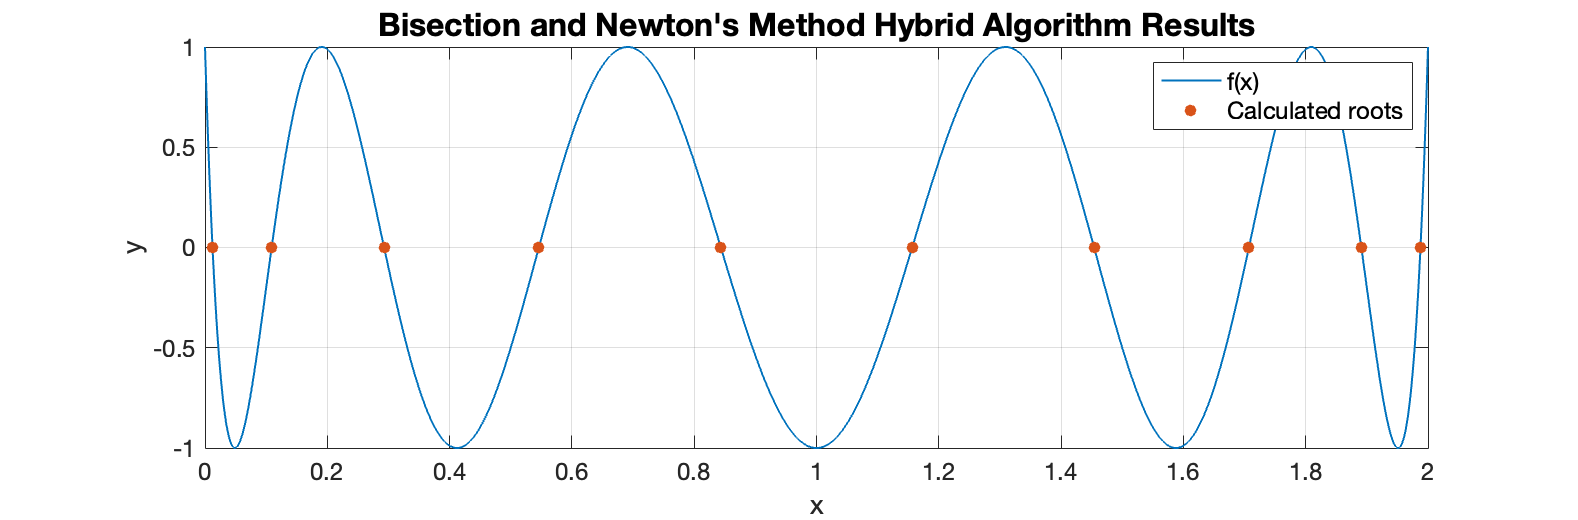
\includegraphics[width=1\textwidth]{HybridPlot.png}
\caption{Numerically calculated roots overlaid on example function $f(x)$.}
\end{figure}

\pagebreak

%%%%%%%%%%%%%%%%%%%%%%%%%%%%%%%%%%%%%%%%%%%%%%%%%%%%%%%%%%%%%%%%%%%%%%%%%%%%%%%%%%%%%%%%%%%%%%%%%%%%%%%
% Problem 2 - D-dimesional Newton's Method
%%%%%%%%%%%%%%%%%%%%%%%%%%%%%%%%%%%%%%%%%%%%%%%%%%%%%%%%%%%%%%%%%%%%%%%%%%%%%%%%%%%%%%%%%%%%%%%%%%%%%%%
\subsection*{Problem 2 - D-dimesional Newton's Method}

\subsubsection*{Review of Theory}

Newton's method in d-dimensions follows the same process as Newton's method in one dimension, however 
the derivative $f'(x)$ is replaced with the Jacobian matrix of $\mathbf{f}(\mathbf{x})$. In order to 
solve $\mathbf{f}(\mathbf{x})=\mathbf{0}$, the multivariate Taylor series expansion is used:
$$\mathbf{0} \approx \mathbf{f}(\mathbf{x}^{(n)}) + \mathbf{J}[\mathbf{x}^{(n)}](\mathbf{x}^* -
\mathbf{x}^{(n)})$$

where

\[
\mathbf{J}_{i,j} =
\begin{bmatrix}
  \frac{\partial f_1}{\partial x_1} & 
    \frac{\partial f_1}{\partial x_2} & 
    \frac{\partial f_1}{\partial x_3} \\[1ex] % <-- 1ex more space between rows of matrix
  \frac{\partial f_2}{\partial x_1} & 
    \frac{\partial f_2}{\partial x_2} & 
    \frac{\partial f_2}{\partial x_3} \\[1ex]
  \frac{\partial f_3}{\partial x_1} & 
    \frac{\partial f_3}{\partial x_2} & 
    \frac{\partial f_3}{\partial x_3}
\end{bmatrix}
\]

Replacing $\mathbf{x}^*$ with $\mathbf{x}^{(n+1)}$:
$$\mathbf{0} \approx \mathbf{f}(\mathbf{x}^{(n)}) + \mathbf{J}[\mathbf{x}^{(n)}](\mathbf{x}^{(n+1)} -
\mathbf{x}^{(n)})$$

An update vector is defined to be $\mathbf{\delta x^{(n)}} = -(\mathbf{x}^{(n+1)}-\mathbf{x}^{(n)})$ that
satisfies the linear system 
$$\mathbf{J}[\mathbf{x}^{(n)}]\mathbf{\delta x^{(n)}} = \mathbf{f}(\mathbf{x}^{(n)})$$

The d-dimensional Newton's method can be iterated until the update vector $\mathbf{\delta x^{(n)}}$ has 
been reduced to a suitably chosen relative precision. 

\subsubsection*{Numerical approach}

The d-dimensional Newton's method algorithm was implemented as a function (as per the homework instructions):
\begin{verbatim}
function x = newtond(f, jac, x0, tol)
\end{verbatim}
where \code{x} is the estimate of the root, \code{f} is the function which implements the nonlinear system of 
equations, \code{jac} is the Jacobian of the nonlinear system, \code{x0} is the initial estimate for the Newton
iteration, and \code{tol} is convergence criterion for the relative magnitude of the update vector.

In order to test the function the following nonlinear system was provided: 
$$x^2+y^4+z^6=2$$
$$\cos{xyz^2}=x+y+z$$
$$y^2+z^3=(x+y-z)^2$$
Putting this into standard form:
$$f_1(\mathbf{x})=x^2+y^4+z^6-2$$
$$f_2(\mathbf{x})=\cos{xyz^2}-x+y+z$$
$$f_3(\mathbf{x})=y^2+z^3-(x+y-z)^2$$

A function in \code{test.m} implemented these equations to be passed as \code{f} to the function \code{newtond}.
The Jacobian was calculated using and online
\href{https://www.emathhelp.net/en/calculators/calculus-3/jacobian-calculator/}{Jacobian calculator} as:

\begin{figure}[h!]
\centering
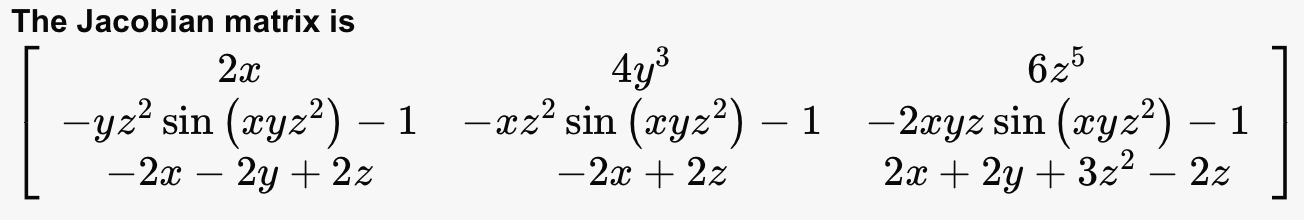
\includegraphics[width=0.75\textwidth]{Jacobian.png}
\caption{Calculated Jacobian matrix for the provided system of equations.}
\end{figure}

This Jacobian was implemented as another function in \code{test.m} to be passed as \code{jac} to the function 
\code{newtond}. As in the problem instructions, $(x, y, z) = (-1.00, 0.75, 1.50)$ was used as an initial guess
and \code{tol} was passed as $10^{-12}$.

Refer to Appendix C for the full Matlab test script. 

\subsubsection*{Implementation}

The d-dimensional Newton iteration was implemented as a while loop that computes the update vector 
\code{dx = jac(x)}\textbackslash\code{res;} where \code{res = f(x0);} each iteration. The \textbackslash\ character 
in Matlab performs matrix left division which immediately solves the system
$$\mathbf{J}[\mathbf{x}^{(n)}]\mathbf{\delta x^{(n)}} = \mathbf{f}(\mathbf{x}^{(n)})$$ for $\mathbf{\delta x^{(n)}}$.
The next approximation to the solution of the system of equations is then found using \code{x = x - dx;}. The loop 
continues until the convergence criterion is reached: \code{rms(dx) > tol}. A loop iteration counter is utilized that
causes the function to immediately return \code{NaN} if the loop exceeds 50 iterations.

Refer to Appendix B for the full Matlab script.

\subsubsection*{Results}

Using the script \code{test.m} shown in Appendix C, the solution of the nonlinear system was computed 
as shown:
\begin{verbatim}
x = -0.577705133337 
y = 0.447447204972 
z = 1.084412371725 
\end{verbatim}

To check that these values are accurate, they were plugged back into the system by computing
$f_1(\mathbf{x})$, $f_2(\mathbf{x})$, and $f_3(\mathbf{x})$, producing the following output:
\begin{verbatim}
system_at_solution =

    1.0e-15 *
   -0.222044604925031
                  0
   -0.444089209850063
\end{verbatim}

This allows us to confirm the values for $x$, $y$, and $z$ are all accurate to the desired relative precision.

\pagebreak

%%%%%%%%%%%%%%%%%%%%%%%%%%%%%%%%%%%%%%%%%%%%%%%%%%%%%%%%%%%%%%%%%%%%%%%%%%%%%%%%%%%%%%%%%%%%%%%%%%%%%%%
% Conclusions
%%%%%%%%%%%%%%%%%%%%%%%%%%%%%%%%%%%%%%%%%%%%%%%%%%%%%%%%%%%%%%%%%%%%%%%%%%%%%%%%%%%%%%%%%%%%%%%%%%%%%%%
\subsection*{Conclusions}

In this homework assignment, functions for a hybrid bisection-Newton's method algorithm in one dimension 
and a Newton's method algorithm in d-dimensions were developed. These functions were tested using an example 
10th order polynomial and nonlinear system of three variables and were found to be correct. 

Generative AI was not used for any part of this homework assignment. 

\pagebreak

%%%%%%%%%%%%%%%%%%%%%%%%%%%%%%%%%%%%%%%%%%%%%%%%%%%%%%%%%%%%%%%%%%%%%%%%%%%%%%%%%%%%%%%%%%%%%%%%%%%%%%%
% Appendix A - Hybrid Algorithm Code
%%%%%%%%%%%%%%%%%%%%%%%%%%%%%%%%%%%%%%%%%%%%%%%%%%%%%%%%%%%%%%%%%%%%%%%%%%%%%%%%%%%%%%%%%%%%%%%%%%%%%%%
\subsection*{Appendix A - Hybrid Algorithm Code}
\lstinputlisting{../hybrid.m}

\pagebreak

%%%%%%%%%%%%%%%%%%%%%%%%%%%%%%%%%%%%%%%%%%%%%%%%%%%%%%%%%%%%%%%%%%%%%%%%%%%%%%%%%%%%%%%%%%%%%%%%%%%%%%%
% Appendix B - D-dimesional Newton's Method Code
%%%%%%%%%%%%%%%%%%%%%%%%%%%%%%%%%%%%%%%%%%%%%%%%%%%%%%%%%%%%%%%%%%%%%%%%%%%%%%%%%%%%%%%%%%%%%%%%%%%%%%%
\subsection*{Appendix B - D-dimesional Newton's Method Code}
\lstinputlisting{../newtond.m}

\pagebreak

%%%%%%%%%%%%%%%%%%%%%%%%%%%%%%%%%%%%%%%%%%%%%%%%%%%%%%%%%%%%%%%%%%%%%%%%%%%%%%%%%%%%%%%%%%%%%%%%%%%%%%%
% Appendix C - Testing Code
%%%%%%%%%%%%%%%%%%%%%%%%%%%%%%%%%%%%%%%%%%%%%%%%%%%%%%%%%%%%%%%%%%%%%%%%%%%%%%%%%%%%%%%%%%%%%%%%%%%%%%%
\subsection*{Appendix C - Testing Code}
\lstinputlisting{../test.m}


\end{document}